\section{References}

\begin{frame}
  \frametitle{Books}
  \begin{columns}
    \column{0.8\textwidth}
    \small
    \begin{itemize}
    \item {\bf Embedded Linux Primer, Second Edition, Prentice Hall}\\
      By Christopher Hallinan, October 2010\\
      Covers a very wide range of interesting topics.\\
      \url{http://j.mp/17NYxBP}
    \item {\bf Building Embedded Linux Systems, O'Reilly}\\
      By Karim Yaghmour, Jon Masters, Gilad Ben-Yossef, Philippe
      Gerum and others (including Michael Opdenacker), August 2008\\
      \url{http://oreilly.com/catalog/9780596529680/}
    \item {\bf Embedded Linux System Design and Development}\\
      P. Raghavan, A. Lad, S. Neelakandan, Auerbach, Dec. 2005.
      Very good coverage of the POSIX programming API (still up
      to date).\\
      \url{http://j.mp/19X8iu2}
    \end{itemize}
    \normalsize
    \column{0.2\textwidth}
    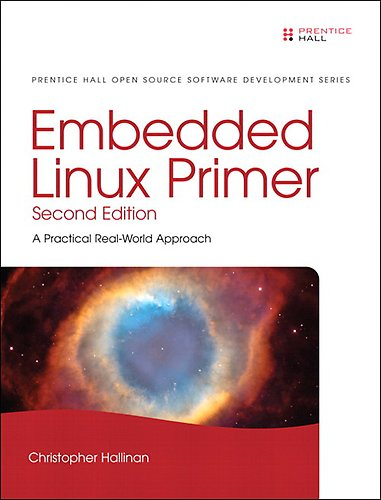
\includegraphics[width=0.7\textwidth]{slides/sysdev-embedded-linux/book-embedded-linux-primer2.jpg}\\
    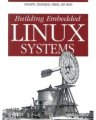
\includegraphics[width=0.7\textwidth]{slides/sysdev-embedded-linux/book-building-embedded-linux-systems.png}\\
    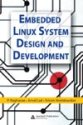
\includegraphics[width=0.7\textwidth]{slides/sysdev-embedded-linux/book-embedded-linux-sysdev.png}\\
  \end{columns}
\end{frame}

\begin{frame}
  \frametitle{Web sites}
  \begin{itemize}
  \item {\bf ELinux.org}, \url{http://elinux.org}, a Wiki entirely
    dedicated to embedded Linux. Lots of topics covered: real-time,
    filesystem, multimedia, tools, hardware platforms,
    etc. Interesting to explore to discover new things.
  \item {\bf LWN}, \url{http://lwn.net}, very interesting news site
    about Linux in general, and specifically about the kernel. Weekly
    newsletter, available for free after one week for non-paying
    visitors.
  \item {\bf Linux Gizmos}, \url{http://linuxgizmos.com}, a news site
    about embedded Linux, mainly oriented on hardware platforms
    related news.
  \end{itemize}
\end{frame}

\begin{frame}
  \frametitle{International conferences}
  Useful conferences featuring embedded Linux and kernel topics
  \begin{itemize}
  \item Embedded Linux Conference: \url{http://embeddedlinuxconference.com/}\\
    Organized by the Linux Foundation: California (Spring), in Europe (Fall).
    Very interesting kernel and user space topics for embedded systems developers.
    Presentation slides freely available
  \item Linux Plumbers, \url{http://linuxplumbersconf.org}\\
    Conference on the low-level plumbing of Linux: kernel, audio,
    power management, device management, multimedia, etc.
  \item FOSDEM: \url{http://fosdem.org} (Brussels, February)\\
    For developers. Presentations about system development.
  \item Don't miss our free conference videos on
    \url{http://free-electrons.com/community/videos/conferences/}!
  \end{itemize}
\end{frame}
